\documentclass{article}
\usepackage{graphicx}
\setlength{\parindent}{0cm}

\usepackage{listings}
\usepackage{color}

\definecolor{dkgreen}{rgb}{0,0.6,0}
\definecolor{gray}{rgb}{0.5,0.5,0.5}
\definecolor{mauve}{rgb}{0.58,0,0.82}

\lstset{frame=tb,
  language=Matlab,
  aboveskip=3mm,
  belowskip=3mm,
  showstringspaces=false,
  columns=flexible,
  basicstyle={\small\ttfamily},
  numbers=none,
  numberstyle=\tiny\color{gray},
  keywordstyle=\color{blue},
  commentstyle=\color{dkgreen},
  stringstyle=\color{mauve},
  breaklines=true,
  breakatwhitespace=true
  tabsize=3
}

\begin{document}

\title{Neural Networks}
\author{Barney Tannahill and Kyle Kastner}

\maketitle

\section*{Cancer Dataset}
The data set used for this exercise consists of 569 different breast cancer diagnoses.
Each diagnosis contains 30 additional measurement parameters. 

\section*{Feedforward Neural Network Classification}
Figure ~\ref{fig:f0} shows the distribution of samples between the two diagnoses 
with the dimension of the data reduced to two in order to better display the data.
\begin{figure}[h!]
\caption{Distribution of samples}
  \centering
    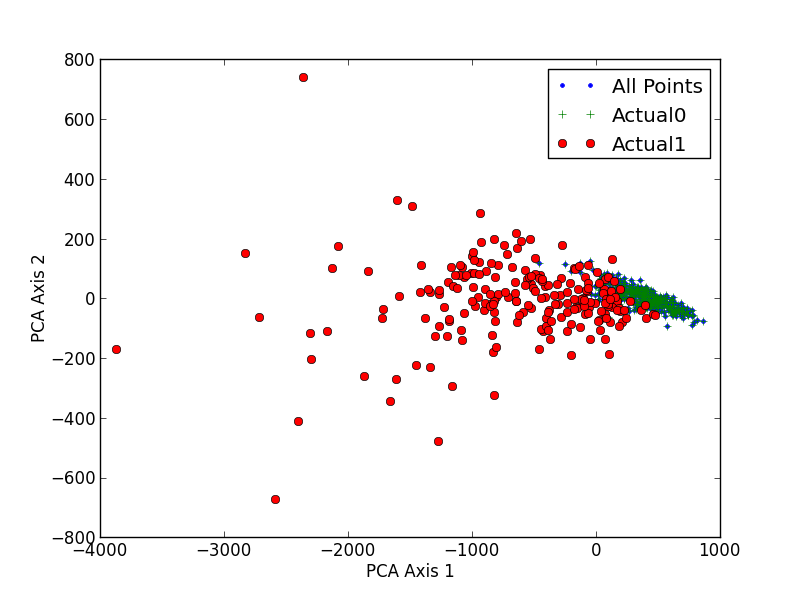
\includegraphics[width=0.85\textwidth]{figure_0.png}
  \label{fig:f0}
\end{figure}
In an attempt to generate a classification method to identify benign and malignant diagnoses
based solely on the gathered parameters, the Feedforward Neural Network algorithm 
available from the neurolab library was used.  The network was chosen to have a single
hidden layer of perceptrons and a single output perceptron.

It was decided that 60\% of the data would be used to train the neural network. 
Figure ~\ref{fig:f1} shows the training profile, showing the Sum Squared Error (SSE) of the network decreasing over the training epochs.
\begin{figure}[h!]
\caption{Training Profile}
  \centering
    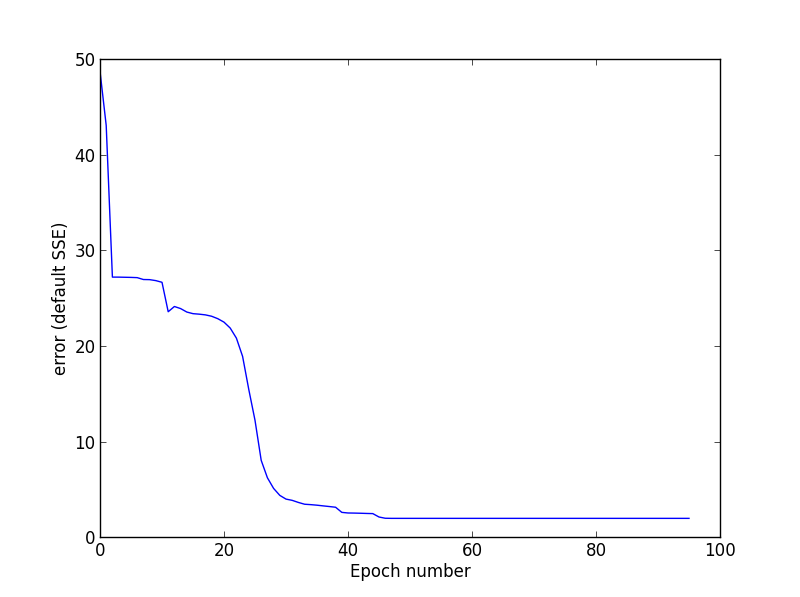
\includegraphics[width=0.85\textwidth]{figure_1.png}
  \label{fig:f1}
\end{figure}

These additional statistics were calculated to help show the effectiveness of the method 
at classifying the diagnosis data as benign or malignant.  For the statistics below,
if the neural network output was greater than 0.5, the test result was counted as a
malignant indication, and if the output was less than 0.5, the result was counted as a benign indication.
\vspace*{1\baselineskip}      
\begin{verbatim}
True Malignant Identification (%): 0.981
False Malignant Identification (%): 0.019
True Benign Identification (%): 0.983
False Benign Identification (%): 0.017
\end{verbatim}
\vspace*{1\baselineskip}      
These statistics show that the categorization is accurate at classifying both malignant and benign diagnosis samples.
Figure ~\ref{fig:f2} shows the same data as Figure ~\ref{fig:f0}, but the data is separated based 
on the output of the neural network.  It can be seen that only minimal differences are present,
again demonstrating the accuracy of the neural network classification method.
\begin{figure}[h!]
\caption{Network Results}
  \centering
    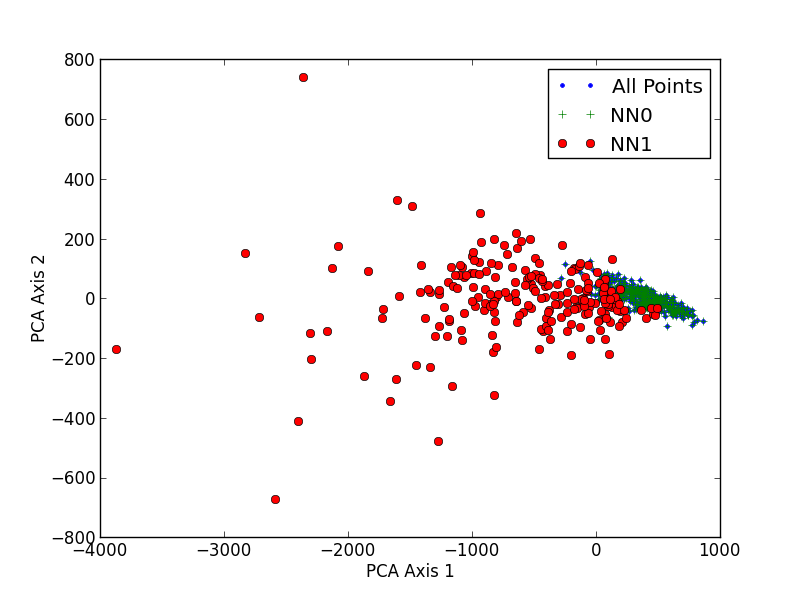
\includegraphics[width=0.85\textwidth]{figure_2.png}
  \label{fig:f2}
\end{figure}

\section*{Object Recognition}
Convolutional neural networks were used to perform object recognition on two different datasets
Each set contains 60000 images with 10 separate classes.
The MNIST dataset is made handwritten digits (0 - 9) in greyscale, with each image size 28x28 pixels.
The CIFAR10 dataset is made of tiny color images (RGB), with each image size 32x32 pixels. The classes 
for the CIFAR10 datset are shown below.
\vspace*{1\baselineskip}      
\begin{verbatim}
airplane
automobile
bird
cat
deer
dog
frog
horse
ship
truck
\end{verbatim}
\vspace*{1\baselineskip}      
The current state of the art for CIFAR10 on unaugmented data is 18\%. Our best result to date
does not match this, but there are further optimizations to be made. Our MNIST unaugmented data results match the state of the art.
\vspace*{1\baselineskip}      
\begin{verbatim}
CIFAR10 1 Layer:0.31
CIFAR10 2 Layer:0.28
CIFAR10 3 Layer:0.25
MNIST 2 Layer:0.0069
\end{verbatim}
\vspace*{1\baselineskip}      
\begin{figure}[h!]
    \caption{CIFAR10 Training Schedule}
  \centering
    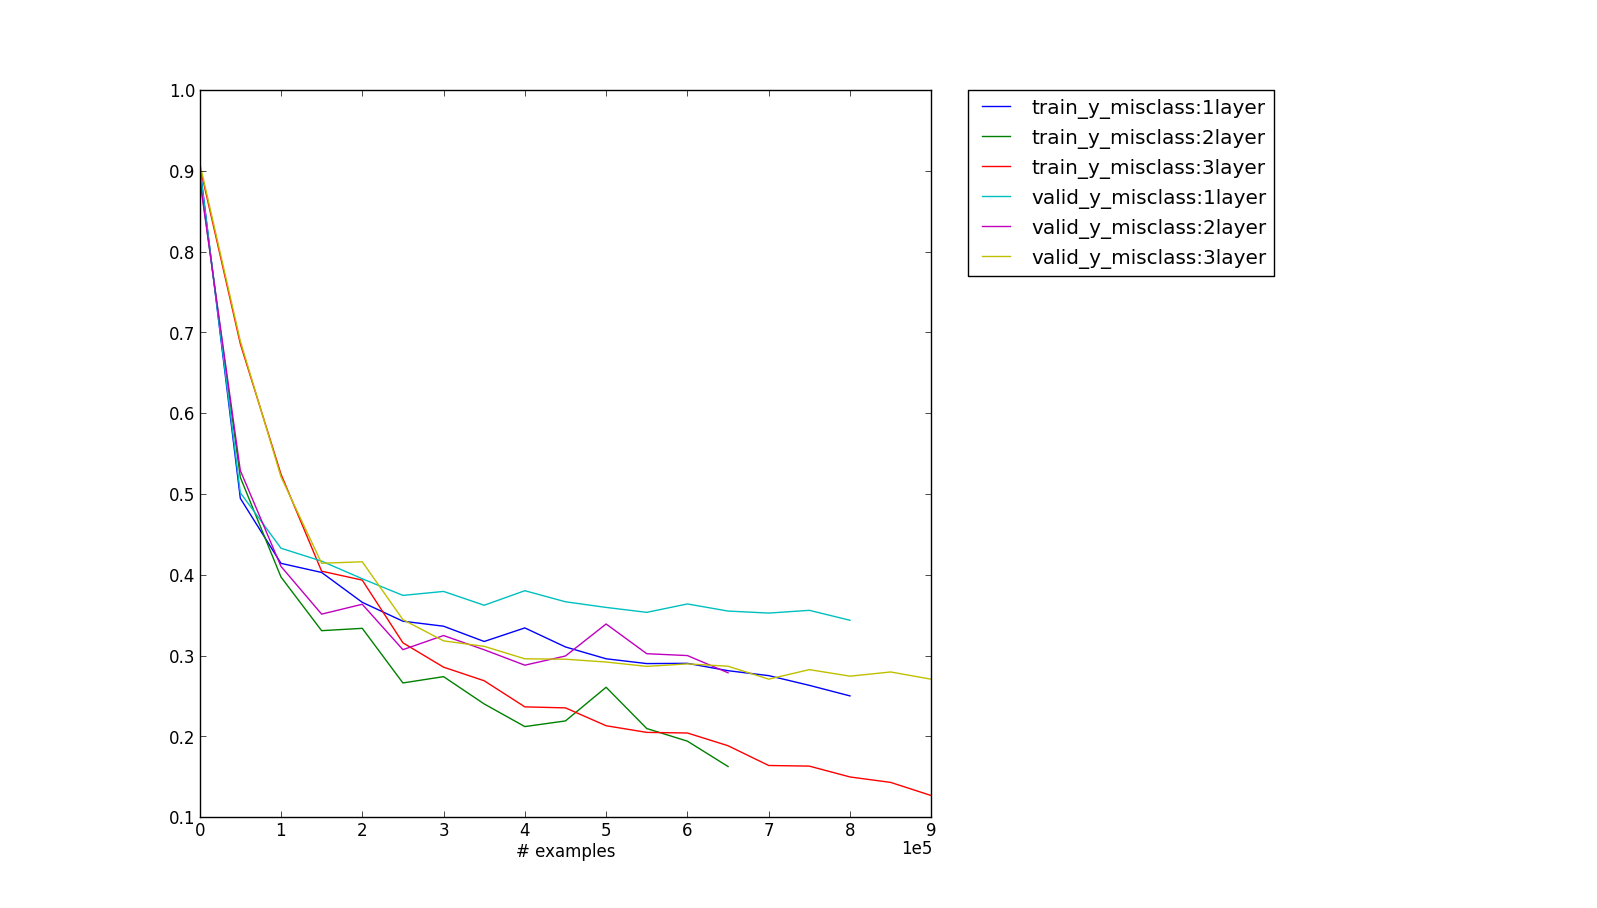
\includegraphics[width=0.85\textwidth]{figure_3.png}
  \label{fig:f3}
\end{figure}
\begin{figure}[h!]
    \caption{CIFAR10 Learned Filters}
  \centering
    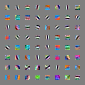
\includegraphics[width=0.85\textwidth]{figure_4.png}
  \label{fig:f4}
\end{figure}
\begin{figure}[h!]
    \caption{MNIST Training Schedule}
  \centering
    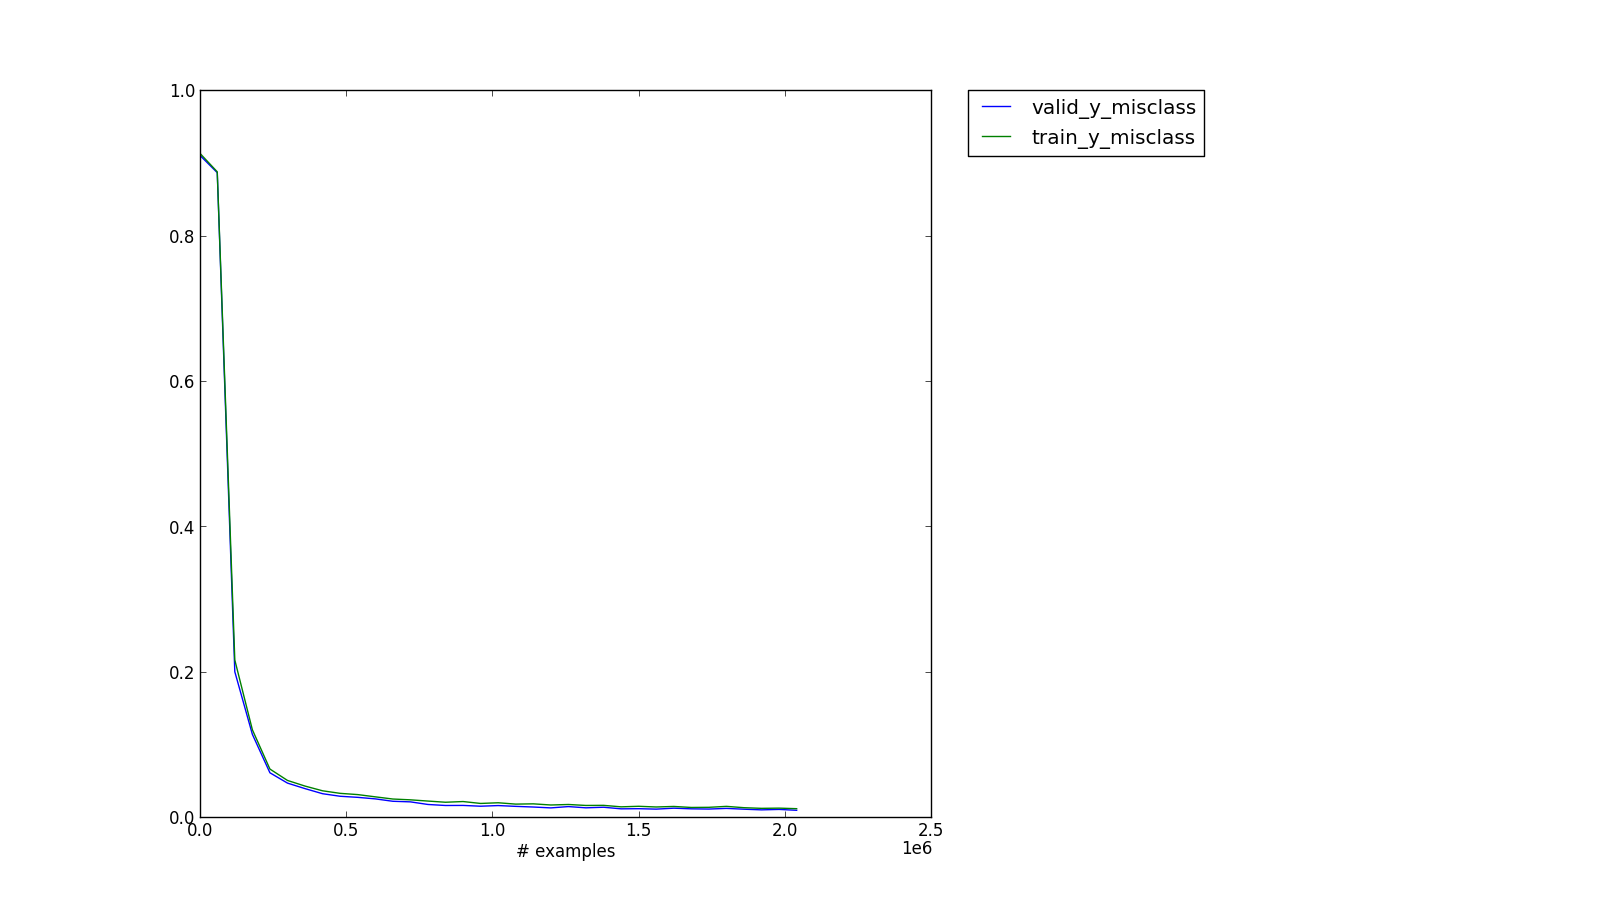
\includegraphics[width=0.85\textwidth]{figure_5.png}
  \label{fig:f5}
\end{figure}
\begin{figure}[h!]
    \caption{MNIST Learned Filters}
  \centering
    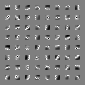
\includegraphics[width=0.85\textwidth]{figure_6.png}
  \label{fig:f6}
\end{figure}

\begin{thebibliography}{9}
\bibitem{BCDiagnostic}
  Dr. William H. Wolberg, W. Nick Street, Olvi L. Mangasarian 
  \emph{Breast Cancer Wisconsin (Diagnostic) Data Set}
  UCI Machine Learning Repository 
  http://archive.ics.uci.edu/ml/datasets/Breast+Cancer+Wisconsin+i\%28Diagnostic\%29
                                                                                        
\bibitem{skfuzzy}
  \emph{Sci-kit Fuzzy Library}
  https://github.com/scikit-fuzzy                       
                                                                                        
\bibitem{iris}
    \emph{Comparison of LDA and PCA 2D projection of Iris Dataset}
    http://scikit-learn.org/stable/auto\_examples/decomposition/plot\_pca\_vs\_lda.html\#example-decomposition-plot-pca-vs-lda-py

\bibitem{neurolab}
    https://code.google.com/p/neurolab

\bibitem{cifar10}
    A. Krizhevsky
    \emph{Learning Multiple Layers of Features from Tiny Images, 2009}
    http://www.cs.toronto.edu/\textasciitilde kriz/cifar.html

\bibitem{mnist}
    Y. LeCun, C. Cortes, C. Burges
    \emph{The MNIST database of handwritten digits}
    http://yann.lecun.com/exdb/mnist/
                                                                                        
\end{thebibliography}
\end{document}
